\documentclass[a4paper]{article}

\usepackage[english]{babel}
\usepackage[utf8]{inputenc}
\usepackage{amsmath}
\usepackage{graphicx}
\usepackage[colorinlistoftodos]{todonotes}
\usepackage[T1]{fontenc}	%ADDED for << og >>

\title{Assinment40}

\author{pebj, smot}

\date{\today}

\begin{document}
\maketitle

\section{Part I - OOSE}

\subsection{Mapping subsystems to processors and components}

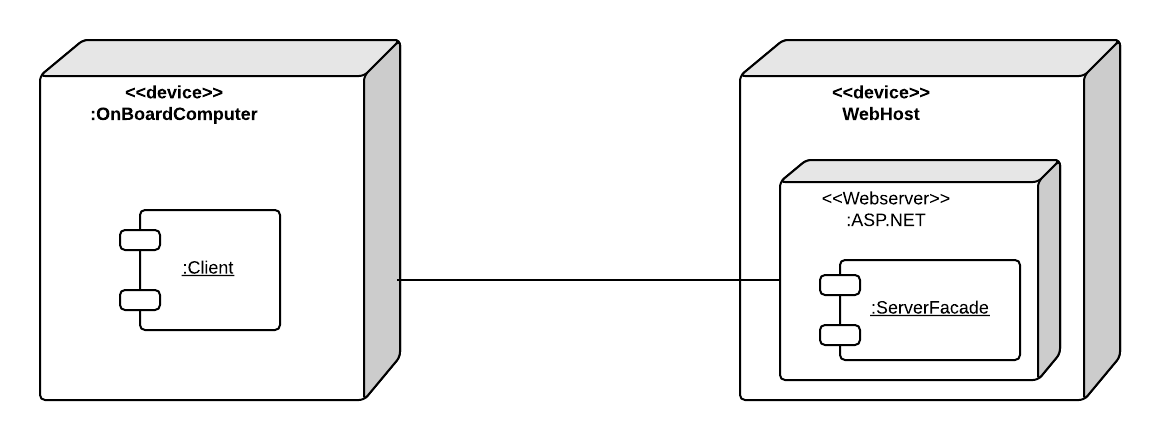
\includegraphics[scale = 0.3]{MappingSubsystems.png}

\subsection{Identifying and storing persistent data}

\textit{\textbf{Identifying persistent objects}}\\

CALENDAR deals with two set of objects that must be stored, the first set involves the Account and the second involves events and notifications. Accounts are created and accessed by the server; however a client will retrieve his own account when his login is authorized by the server. Events and notifications however are stored on both the server and client and will seek to synchronize with one another when there is internet connection. Therefore all persistent objects of a client is a subset of the objects on the server associated with a specific account. Here is a table that shows with classes there is responsible for storing. Table \ref{tab:stored}.  \\

\begin{table}
\centering

\begin{tabular}{l l}
	\hline\\
	\multicolumn{2}{l}{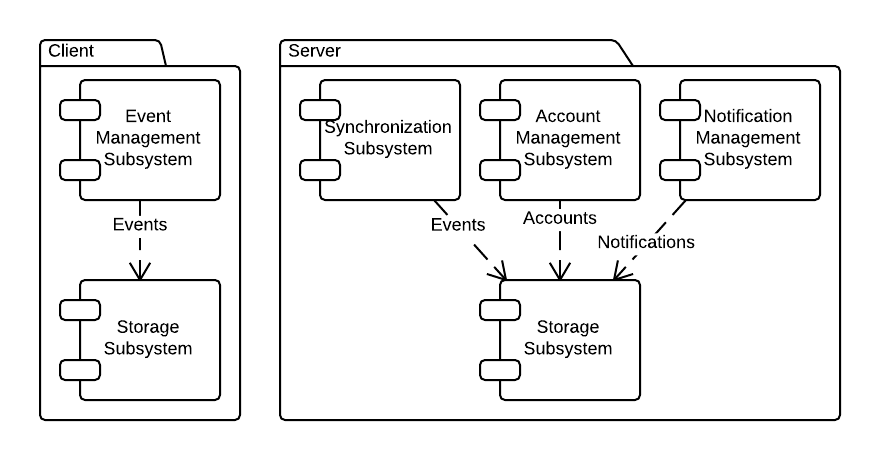
\includegraphics[scale = 0.3]{StoregetModel.png}}\\

	\textbf{EventManagementSubsystem}	&The EventManagementSubsystem\\
    									&instantiate new Events as\\
                                        &specified by the user, and\\
                                        &receives Events given by the\\
                                        &SynchronizationSubsystem to\\
                                        &store on the local pc\\
                                        &\\
	\textbf{SynchronizationSubsystem}	&The SynchronizationSubsystem resives\\
    									&Events and stores them and can give\\
                                        &the needet Events for Synchronization.\\
                                        &\\
	\textbf{StorageSubsystem}			&The two StorageSubsystem is the same\\
    									&subsystem but to different instances.\\
	\hline
\end{tabular}

\caption{authentication and storing user data}
\label{tab:stored}

\end{table}


\textit{\textbf{Selecting a storage strategy}}\\

The assignment has a demand for support of 3 different storage methods: test stub, file storage, and a RDBMS storage. There should be synchronization between that and an external server like “Google Calendar”. Since we want a notification feature, it will be required that a server will run a script forever that checks for upcoming notification dates and sends out emails. For this reason, we will need the client software to synchronize notification data with a script we make on a server. Just like with the client, we will enable the support for the same 3 different storage methods on that server. The server will also synchronize events with the client and do account validation for the client.  There is also a demand for the command pattern in the solution, and we can use that for efficiency of synchronization between the server/client’ storage. A client holds commands that once the client goes online, will be sent to the server. Likewise, the client’ storage will be updated accordingly by sending the server the timestamp for the last time it synchronized (this timestamp is received from the server’ timestamp when it receives response from it). Any field in the database with a timestamp later than a given timestamp will be sent to the client/server in the form of commands to update their storage. If a command is never than what it tries to change, it will update the persistent data of either the client or server. In other words, persistent time values will keep track of what needs to be handled. This will minimize the stress on internet traffic, thus lowering server costs.\\

\textbf{Pros}
\begin{enumerate}
\item Because of the command pattern, the user won't lose changes during synchronization if he has synchronized other changes from another computer.
\item Using local storage enables the system to work offline and won't require a user to wait for a server to respond when during daily activities.
\item Command pattern and timestamps enables us to minimize traffic to/from server and client by not transfering the entire storage between synchronization. This could mean lower server costs.
\end{enumerate}

\textbf{Cons}
\begin{enumerate}
\item A server is required to run at all times. Downtime means that clients won't receive notifications.
\item If the differences between client and server storage is significiant, it might require the client to wait a while before he sees the events he awaits. This could happen if he migrated to another computer and had to synchronize the entire storage with the server.
\end{enumerate}


\subsection{Providing access control}
\label{sec:accessControl}
  
  
CALENDAR's server have to manages multible users request for data and storig ther data on a database thad introduces security issues. We most ensure the only authorized user get ther own data. The model for this can be seen in Table \ref{tab:auther}.\\
  
\begin{table}
\centering

\begin{tabular}{l l}
	\hline
	\textbf{ClientSubsystem}	&The ClientSubsystem is responsible for representing\\
    							&the user in communication with the server, and therefore\\
                                &sending account data with each request.\\
    \hline
	\textbf{AccountManagement}	&The AccountManagementSubsystem is responsible for\\
    \textbf{Subsystem}			&identifying and updating Accounts. Prior to processing any\\
                                &requests, the AccountManagementSubsystem authentication\\
                                &the Account from the ServerFacadeSubsystem.\\
	\hline
	\textbf{Account}			&A Account contains identifying informations about a\\
    							&authenticated user. A copy is stored by the Client\\
    							&Subsystem when the user is loggetin. The\\
                                &AccountManagement Subsystem identify the Account.\\
	\hline
\end{tabular}

\caption{authentication and storing user data}
\label{tab:auther}

\end{table}
 
Providing accesscontrol is all about notating who has permission to which permissions on objects and who creates the objects. Below we have an accessmatrix describing the operations allowed by each actor. For summary, a user can create/access and edit the account/events and eventnotifications associated with the specific account. A moderator actor however has access to all accounts and their events and notifications. A moderator has permission to do everything including removal of a user’ account. Lastly we have the server actor who sends notification emails to users. It only needs access to the user’ email and upcoming notifications. Table \ref{tab:ObjectsActors}.\\

\begin{table}
\centering

\begin{tabular}{l | l | l | l}
	\hline
	Objects Actors	&Account 	&Event 			&Notification\\
	\hline
	User		&<<create>>		&<<create>>		&<<create>>\\
    			&CreateAccount	&CreateEvent	&CreateNotification\\
                &GetAccount		&EditEvent		&EditNotification\\
                &EditAccount	&DeleteEvent	&\\
    \hline
	Moderator 	&GetAccounts	&<<create>>		&\\
    			&GetAccount		&CreateEvent	&\\
                &DeleteAccount	&EditEvent		&\\
                &EditAccount	&DeleteEvent	&\\
	\hline
	Webservice	&GetEmail		& 				&GetUpcommingNotifications\\
	\hline
\end{tabular}

\caption{Accessmatrix}
\label{tab:ObjectsActors}

\end{table}

\subsection{Designing the global control flow}

Designing the global control flow
During the design of "access control" and "object model" we greatly restricted how the code should be centralized. The control flow will generally be event driven since any action made by the client to change/create account or events will be dispatched to the appropriate methods of either AccountManagement and EventManagement. Here the correct commands will also be created and added to to a query of what needs to be dispatched to the server/storage during synchronization.
Another point of view is that each request of the webserver has its own thread on the server. When a client dispatches commands to the server, the server will trigger the right function depending on the type of command resulting in an event driven logic. A client can also share events with other users, so a client can trigger an event to happen in a specific client, namely the creation of the shared event in his calendar.  The idea of each request having its own thread makes it possible for the webserver to handle multiple users simultaniously. Without that, a user might have had to wait days to get a turn on the server if the system had enough users. The flow from when a client asks the webserver to do something can be said to be thread driven. A thread will be assigned to a each client on the server and each thread can affect the outcome of the others.

When we talk about the client again, all user interfaces will also be event driven (buttons etc.). \\


\subsection{Identifying services}

Being that we have different actors as shown in Table \ref{tab:ObjectsActors}, it is nessesary to implement an authorization service to authorize a user’ rights. The moderator and client are both using the same software, so a authorization check between a client and server is necessary. This is also to prevent a client from having access to other users account data as described in section \ref{sec:accessControl}. A client will ask a server if an account is valid and only then will the sever allow access or modification of accounts and synchronization storage.
We will also need a storage service which creates the commands to be used by the command pattern for changes requested by eventmanagement and accountmanagement. The service’ job is to centralize command codes and to have it give them over to the synchronization service.
Lastly we will have a service for the webservice who continuesly checks up on active notifications to find out who needs to be sent an email. This service will run forever.\\

LISTING AF SERVICES OG DIAGRAM..\\

\subsection{Identifying boundary conditions}

\textbf{Start-up and shutdown use cases.}\\

Client:
	Start-up,
    shutdown,
    Configuration\\
    
WebServis:
	Start-up,
    shutdown,
    Configuration\\

*Deadline!

\textbf{Exception handling use cases.}\\

network outage Table \ref{tab:Network}\\

\begin{table}
\centering
\begin{tabular}{l r l}
	\multicolumn{2}{c}{} \\
	\hline
	\textit{Use case name:}		&\multicolumn{2}{l}{Network outage} \\
    \hline
	\textit{Entry condition:}		&1.&The Network stops responting to the Client.\\
	\hline
	\textit{Flow of events:}		&2.&The Client stops waiting for response and notifies the user.\\
						&3.&The Client commits new changes to the local storage.\\
	\hline
	\textit{Exit condition:}		&4.&The Client checks the last synchronization timestamp,\\
							&& and restore changes made after.\\
	\hline
\end{tabular}
\caption{Network outage use case}
\label{tab:Network}
\end{table}

\subsection{UML diagram of the prototype}

\begin{figure}
\centering
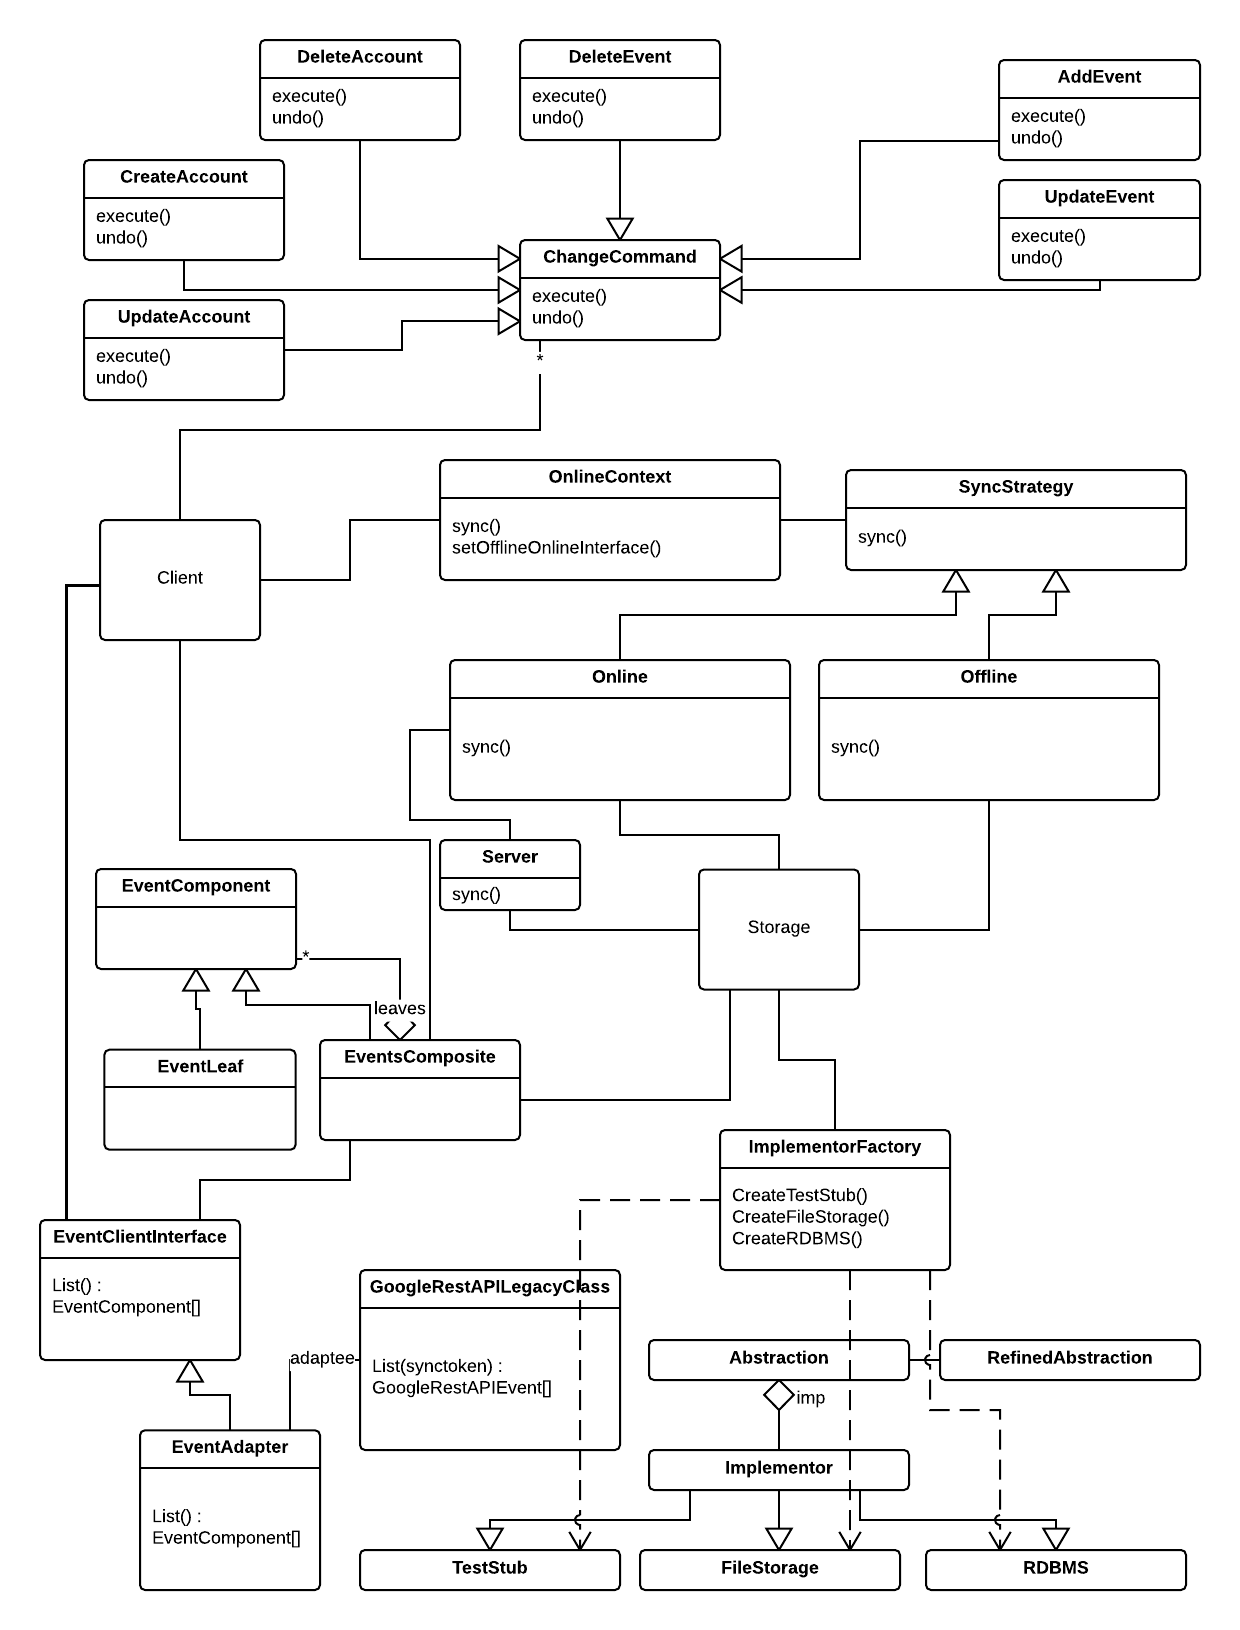
\includegraphics[scale = 0.3]{C:/Users/stin7054/Documents/GitHub/BDSA2014/LatexAS.40/Prototype.png}
\caption{CShap Prototype model of design patterns}
\label{fig:Prototype}
\end{figure}

Figure \ref{fig:Prototype} describes the classes nessesary to have a ''bridge'', ''adapter'', ''strategy'', ''Abstract factory'', ''Composite'' and ''Command'' pattern. A bridge allows for using between using a ''test stub'', ''filestorage'' and ''RDBMS'' storage and the ''abstract factory'' allows for the creation of one of the storagemethods. ''Adapter pattern'' allows us to retain our event structure when we get a list of events from Google Rest API, the adapter converts Google Rest API events to the structure we need. A composite design pattern then allows all events to be handled a specific way and whatever change is made to events or accounts will become the appropriate command to execute on both the offline client and the server connected though the online interface who in responce to synchronization updates the local storage.\\
Figure \ref{fig:Prototype} lacks alot of classes needed for the program itself like the boundaries and there control classes as well as entity classes, but those classes can be seen in the initial analises model we handed in earlier. To illustrate which classes of the above diagram that those closes will speak with, we have drawn a ''Client'' process which simply refers to the client program consisted of the initial analises model.

\end{document}